\let\lesson\undefined
\newcommand{\lesson}{\phantomlesson{Ôn tập chương 9}}
\setcounter{section}{2}
\setcounter{ex}{0}
\Opensolutionfile{ans}[ans/VN10-2023-PH-TP0009-TN]
% ===================================================================
\begin{ex}\mkstar{1}
Lực đàn hồi xuất hiện tỉ lệ với độ biến dạng khi 	
	\choice
	{một vật bị biến dạng dẻo}
	{\True một vật biến dạng đàn hồi}
	{một vật bị biến dạng}
	{ta ấn ngón tay vào một viên đất nặn}
	\loigiai{Lực đàn hồi xuất hiện tỉ lệ với độ biến dạng khi một vật biến dạng đàn hồi.}
\end{ex}
% ===================================================================
\begin{ex}\mkstar{1}
	Kết luận nào sau đây \textbf{không} đúng đối với lực đàn hồi?
	\choice
	{Xuất hiện khi vật bị biến dạng}
	{\True Luôn là lực kéo}
	{Tỉ lệ với độ biến dạng}
	{Ngược hướng với lực làm nó bị biến dạng}
	\loigiai{	Lực đàn hồi có khi là lực kéo, có khi là lực nén.}
\end{ex}
% ===================================================================
\begin{ex}\mkstar{1}
Điều nào sau đây là \textbf{sai} khi nói về phương và độ lớn của lực đàn hồi?	
	\choice
	{Với cùng độ biến dạng như nhau, độ lớn của lực đàn hồi phụ thuộc vào kích thước và bản chất của vật đàn hồi}
	{Với các mặt tiếp xúc bị biến dạng, lực đàn hồi vuông góc với các mặt tiếp xúc}
	{Với các vật như lò xo, dây cao su, thanh dài, lực đàn hồi hướng dọc theo trục của vật}
	{\True Lực đàn hồi có độ lớn tỉ lệ nghịch với độ biến dạng của vật biến dạng}
	\loigiai{Lực đàn hồi tỉ lệ thuận với độ biến dạng của vật biến dạng.}
\end{ex}
% ===================================================================
\begin{ex}\mkstar{1}
	Khẳng định nào sau đây là đúng khi ta nói về lực đàn hồi của lò xo và lực căng của dây?
	\choice
	{\True Đó là những lực chống lại sự biến dạng đàn hồi của lò xo và sự căng của dây}
	{Đó là những lực gây ra sự biến dạng đàn hồi của lò xo và sự căng của dây}
	{Chúng đều là những lực kéo}
	{Chúng đều là những lực đẩy}
	\loigiai{Lực đàn hồi của lò xo và lực căng của dây: đó là những lực chống lại sự biến dạng đàn hồi của lò xo và sự căng của dây.}
\end{ex}
% ===================================================================
\begin{ex}\mkstar{1}
	Một vật tác dụng một lực vào một lò xo có đầu cố định và làm lò xo biến dạng. Điều nào dưới đây là \textbf{không đúng}?
	\choice
	{Độ đàn hồi của lò xo có độ lớn bằng lực tác dụng và chống lại sự biến dạng của lò xo}
	{Lực đàn hồi cùng phương và ngược chiều với lực tác dụng}
	{\True Lực đàn hồi lớn hơn lực tác dụng và chống lại lực tác dụng}
	{Khi vật ngừng tác dụng lên lò xo thì lực đàn hồi của lò xo cũng mất đi}
	\loigiai{}
\end{ex}
% ===================================================================
\begin{ex}\mkstar{1}
Chọn phát biểu \textbf{sai} về lực đàn hồi của lò xo.	
	\choice
	{Lực đàn hồi của lò xo có xu hướng chống lại nguyên nhân gây ra biến dạng}
	{Lực đàn hồi của lò xo dài có phương là trục lò xo, chiều ngược với chiều biến dạng của lò xo}
	{Lực đàn hồi của lò xo có độ lớn tuân theo định luật Hooke}
	{\True Lực đàn hồi của lò xo chỉ xuất hiện ở đầu lò xo đặt ngoại lực gây biến dạng}
	\loigiai{Lực đàn hồi xuất hiện ở hai đầu của lò xo và tác dụng vào các vật tiếp xúc (hay gắn) với lò xo làm nó biến dạng.}
\end{ex}
% ===================================================================
\begin{ex}\mkstar{1}
Lực đàn hồi của lò xo có tác dụng làm cho lò xo	
	\choice
	{chuyển động}
	{thu gia tốc}
	{\True có xu hướng lấy lại hình dạng và kích thước ban đầu}
	{vừa biến dạng vừa thu gia tốc}
	\loigiai{}
\end{ex}
% ===================================================================
\begin{ex}\mkstar{2}
	Một lò xo có chiều dài tự nhiên là $\SI{20}{cm}$. Khi lò xo có chiều dài $\SI{24}{cm}$ thì lực đàn hồi của nó bằng $\SI{5}{N}$. Hỏi khi lực đàn hồi của lò xo bằng $\SI{10}{N}$ thì chiều dài của nó bằng bao nhiêu?
	\choice
	{$\SI{22}{cm}$}
	{\True $\SI{28}{cm}$}
	{$\SI{40}{cm}$}
	{$\SI{48}{cm}$}
	\loigiai{Ta có:
		$$F = k \Delta l.$$
		Vậy: 
		$$F_1 = k \Delta l_1; F_2 = k \Delta l_2.$$
		Lập tỉ số:
		$$\dfrac{F_1}{F_2} = \dfrac{\Delta l_1}{\Delta l_2} \Rightarrow \Delta l_2 = \SI{0,08}{m} = \SI{8}{cm}.$$
		Chiều dài của lò xo là
		$$l' = l_0 + \Delta l_2 = \SI{28}{cm}.$$}
\end{ex}
% ===================================================================
\begin{ex}\mkstar{2}
	Một lò xo có chiều dài tự nhiên bằng $\SI{22}{cm}$. Lò xo được treo thẳng đứng, một đầu giữ cố định, còn đầu kia gắn một vật nặng. Khi ấy lò xo dài $\SI{27}{cm}$, cho biết độ cứng lò xo là $\SI{100}{N/m}$. Độ lớn lực đàn hồi bằng 	
	\choice
	{$\SI{500}{N}$}
	{\True $\SI{5}{N}$}
	{$\SI{20}{N}$}
	{$\SI{50}{N}$}
	\loigiai{Độ biến dạng của lò xo:
		$$\Delta l = l-l_0 = \SI{5}{cm} = \SI{0,05}{m}.$$
		Độ lớn của lực đàn hồi:
		$$F_\text{đh} = k\Delta l = \SI{5}{N}.$$}
\end{ex}
% ===================================================================
\begin{ex}\mkstar{2}
	Phải treo một vật có khối lượng bằng bao nhiêu vào lò xo có độ cứng $\SI{100}{N/m}$ để lò xo dãn ra được $\SI{10}{cm}$? Lấy $g = \SI{10}{m/s}^2$.
	\choice
	{\True $\SI{1}{kg}$}
	{$\SI{10}{kg}$}
	{$\SI{100}{kg}$}
	{$\SI{1000}{kg}$}
	\loigiai{Ta có: 
		$$F_\text{đh} = k\Delta l = \SI{10}{N}.$$
		Mà $F_\text{đh} = P.$\\
		Suy ra:
		$$m = \dfrac{P}{g} = \SI{1}{kg}.$$}
\end{ex}
	
% ===================================================================
\begin{ex}\mkstar{2}
Dùng một lò xo để treo một vật có khối lượng $\SI{300}{g}$ thì thấy lò xo dãn một đoạn $\SI{2}{cm}$. Nếu treo thêm một vật có khối lượng $\SI{150}{g}$ thì độ dãn của lò xo là	
	\choice
	{$\SI{1}{cm}$}
	{$\SI{2}{cm}$}
	{\True $\SI{3}{cm}$}
	{$\SI{4}{cm}$}
	\loigiai{Khi treo vật khối lượng $\SI{300}{g}$:
		$$m_1g = k\Delta l_1 \Rightarrow k = \dfrac{m_1 g}{\Delta l_1}.$$
		Khi treo thêm một vật ta có:
		$$(m_1+m_2)g = k\Delta l_2 \Rightarrow \Delta l_2 = \dfrac{(m_1+m_2)g}{k} = \SI{0,03}{m} = \SI{3}{cm}.$$}
\end{ex}
% ===================================================================
\begin{ex}\mkstar{2}
	Một lò xo có chiều dài tự nhiên bằng $\SI{20}{cm}$. Khi bị kéo lò xo dài $\SI{24}{cm}$ và lực đàn hồi của nó bằng $\SI{5}{N}$. Hỏi khi lực đàn hồi của lò xo bằng $\SI{15}{N}$ thì chiều dài của nó bằng bao nhiêu?
	\choice
	{$\SI{28}{cm}$}
	{\True $\SI{32}{cm}$}
	{$\SI{45}{cm}$}
	{$\SI{20}{cm}$}
	\loigiai{	Ta có:	
		$$F = k \Delta l.$$	
		Vậy: 
		$$F_1 = k \Delta l_1; F_2 = k \Delta l_2.$$	
		Lập tỉ số:	
		$$\dfrac{F_1}{F_2} = \dfrac{\Delta l_1}{\Delta l_2} \Rightarrow \Delta l_2 = \SI{0,12}{m} = \SI{12}{cm}.$$	
		Chiều dài của lò xo là	
		$$l' = l_0 + \Delta l_2 = \SI{32}{cm}.$$}
\end{ex}

% ===================================================================
\begin{ex}\mkstar{3}
Một lò xo có chiều dài tự nhiên $\ell_0=\SI{27}{\centi\meter}$, được treo thẳng đứng. Khi treo vào một vật có trọng lượng $P_1=\SI{5}{\newton}$ thì lò xo dài $\ell_1=\SI{44}{\centi\meter}$. Khi treo vật khác có trọng lượng $P_2$ chưa biết, lò xo dài $\ell_2=\SI{35}{\centi\meter}$. Độ cứng của lò xo và trọng lượng $P_2$ là	
	\choice
	{$k=\SI{25.3}{\newton/\meter}$, $P_2=\SI{2.35}{\newton}$}
	{\True $k=\SI{29.4}{\newton/\meter}$, $P_2=\SI{2.35}{\newton}$}
	{$k=\SI{25.3}{\newton/\meter}$, $P_2=\SI{3.5}{\newton}$}
	{$k=\SI{29.4}{\newton/\meter}$, $P_2=\SI{3.5}{\newton}$}
	\loigiai{Độ cứng lò xo:
		$$k=\dfrac{P_1}{\ell_1-\ell_0}=\dfrac{\left(\SI{5}{\newton}\right)}{\SI{0.44}{\meter}-\SI{0.27}{\meter}}\approx\SI{29.4}{\newton/\meter}$$
		Trọng lượng $P_2$:
		$$P_2=k\left|\Delta\ell_2\right|=\left(\SI{29.4}{\newton/\meter}\right)\cdot\left|\SI{0.35}{\meter}-\SI{0.27}{\meter}\right|\approx\SI{2.35}{\newton}.$$}
\end{ex}
% ===================================================================
\begin{ex}\mkstar{3}
	Một lò xo có độ cứng $k$, chiều dài tự nhiên $\ell_0$ được treo thẳng đứng, đầu trên cố định. Khi người ta treo quả cân có khối lượng $\SI{200}{\gram}$ vào đầu dưới của lò xo, lò xo có độ dài $\SI{32}{\centi\meter}$. Nếu treo thêm quả cân có khối lượng $\SI{500}{\gram}$ vào đầu dưới của lò xo thì lò xo có chiều dài $\SI{37}{\centi\meter}$. Lấy $g=\SI{10}{\meter/\second^2}$. Độ dài tự nhiên và độ cứng của lò xo là
	\choice
	{$\ell_0=\SI{30}{\centi\meter}$, $k=\SI{1000}{\newton/\meter}$}
	{$\ell_0=\SI{32}{\centi\meter}$, $k=\SI{300}{\newton/\meter}$}
	{$\ell_0=\SI{32}{\centi\meter}$, $k=\SI{2300}{\newton/\meter}$}
	{\True $\ell_0=\SI{30}{\centi\meter}$, $k=\SI{100}{\newton/\meter}$}
	\loigiai{Độ cứng của lò xo:
		$$k=\dfrac{m_2g}{\ell_2-\ell_1}=\dfrac{\left(\SI{0.5}{\kilogram}\right)\cdot\left(\SI{10}{\meter/\second^2}\right)}{\SI{0.37}{\meter}-\SI{0.32}{\meter}}=\SI{100}{\newton/\meter}$$
		Độ biến dạng của lò xo khi treo vật khối lượng $m_1=\SI{200}{\gram}$:
		$$\Delta\ell_1=\dfrac{m_1g}{k}=\SI{0.02}{\meter}=\SI{2}{\centi\meter}$$
		Độ dài tự nhiên của lò xo:
		$$\ell_0=\ell_1-\Delta\ell_1=\SI{30}{\centi\meter}.$$}
\end{ex}
% ===================================================================
\begin{ex}\mkstar{3}
Người ta treo một đầu lò xo vào một điểm cố định, đầu dưới của lò xo là những chùm quả nặng, mỗi quả đều có khối lượng $m$. Khi chùm quả nặng có 2 quả, chiều dài lò xo là $\SI{15}{\centi\meter}$. Khi chùm quả nặng có 4 quả, chiều dài lò xo là $\SI{17}{\centi\meter}$. Cho $g=\SI{10}{\meter/\second^2}$. Số quả nặng cần treo để lò xo dài $\SI{21}{\centi\meter}$ là	
	\choice
	{\True 8 quả}
	{10 quả}
	{6 quả}
	{9 quả}
	\loigiai{Độ biến dạng của lò xo khi treo quả nặng:
		\begin{eqnarray*}
			&&\Delta\ell=\dfrac{mg}{k}\\
			&\Rightarrow& \dfrac{\ell_2-\ell_1}{\ell_3-\ell_1}=\dfrac{\left(m_2-m_1\right)g}{\left(m_3-m_1\right)g}\\
			&\Leftrightarrow& \dfrac{4m-2m}{N\cdot m-2m}=\dfrac{\SI{17}{\centi\meter}-\SI{15}{\centi\meter}}{\SI{21}{\centi\meter}-\SI{15}{\centi\meter}}\\
			&\Rightarrow& N=8.
	\end{eqnarray*}}
\end{ex}
% ===================================================================
\begin{ex}\mkstar{3}
	\immini{Một vật có khối lượng $M$ được gắn vào một dầu của lò xo có độ cứng $k$ được đặt trên mặt phẳng nghiêng góc $\theta$ so với phương ngang, bỏ qua ma sát giữa vật và mặt nghiêng, vật ở trạng thái đứng yên. Độ dãn của lò xo là
	\choice
	{$x=\dfrac{2Mg\sin\theta}{k}$}
	{\True $x=\dfrac{Mg\sin\theta}{k}$}
	{$x=\dfrac{Mg}{k}$}
	{$x=\sqrt{2Mg}$}
	}
	{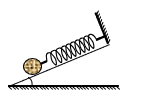
\includegraphics[scale=0.7]{../figs/VN10-2023-PH-TP0009-1}}
	\loigiai{Vật nhỏ cân bằng:
		\begin{equation}
			\label{eq:0009-1}
			\vec P+\vec N+\vec F_\text{đh}=\vec 0
		\end{equation}
		Chiếu phương trình (\ref{eq:0009-1}) lên phương song song măt nghiêng:
		\begin{eqnarray*}
			&&P\sin\theta=F_\text{đh}\\
			&\Leftrightarrow& mg\sin\theta=kx\\
			&\Rightarrow& x=\dfrac{Mg\sin\theta}{k}.
	\end{eqnarray*}}
\end{ex}
% ===================================================================
\begin{ex}\mkstar{3}
\immini{Hai lò xo A và B được bố trí như hình vẽ. Độ cứng của lò xo A là $k_A=\SI{100}{\newton/\meter}$. Khi kéo đầu tự do của lò xo B ra, lò xo A dãn $\SI{5}{\centi\meter}$, lò xo B dãn $\SI{1}{\centi\meter}$. Độ cứng của lò xo B là
\choice
{$\SI{100}{\newton\meter}$}
{$\SI{25}{\newton/\meter}$}
{$\SI{350}{\newton/\meter}$}
{\True $\SI{500}{\newton/\meter}$}
}	
{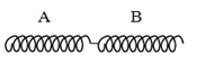
\includegraphics[scale=0.7]{../figs/VN10-2023-PH-TP0009-2}}
	\loigiai{Vì hai lò xo được ghép nối tiếp, lực đàn hồi trên hai lò xo có độ lớn như nhau:
		\begin{eqnarray*}
			&&F_\text{đh A}=F_\text{đh B}\\
			&\Leftrightarrow& \dfrac{k_B}{k_A}=\dfrac{\Delta\ell_A}{\Delta\ell_B}=5\\
			&\Rightarrow& k_B=5k_A=\SI{500}{\newton/\meter}.
	\end{eqnarray*}}
\end{ex}
% ===================================================================
\begin{ex}\mkstar{3}
	\immini{Hai lò xo giống nhau có cùng độ cứng $\SI{100}{\newton/\meter}$ được bố trí như hình vẽ. Vật $m$ có khối lượng $\SI{200}{\gram}$. Khi vật nặng cân bằng, độ dãn của mỗi lò xo là
	\choice
	{\True $\SI{1}{\centi\meter}$}
	{$\SI{2}{\centi\meter}$}
	{$\SI{1.5}{\centi\meter}$}
	{$\SI{3}{\centi\meter}$}
	}
	{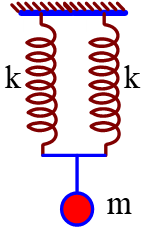
\includegraphics[scale=0.5]{../figs/VN10-2023-PH-TP0009-4}}
	\loigiai{Vật nặng cân bằng:
		$$F_\text{đh 1}+F_\text{đh 2}=mg$$
		$$\Leftrightarrow \Delta\ell=\dfrac{mg}{2k}=\SI{0.01}{\meter}=\SI{1}{\centi\meter}.$$}
\end{ex}
% ===================================================================
\begin{ex}\mkstar{3}
	\immini{Hình bên là đồ thị gồm hai đường thẳng xiên góc đi qua gốc toạ độ $O$, mô tả sự thay đổi giá trị của lực đàn hồi theo các độ dãn khác nhau của lò xo X và lò xo Y. Chọn kết luận đúng về độ cứng của hai lò xo.
	\choice
	{$k_X<k_Y$}
	{$k_X\le k_Y$}
	{$k_X=k_Y$}
	{\True $k_X>k_Y$}
	}
	{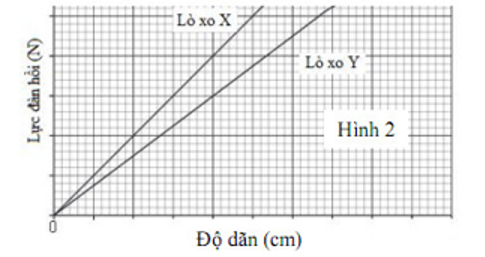
\includegraphics[scale=0.6]{../figs/VN10-2023-PH-TP0009-3}}
	\loigiai{Với cùng độ lớn lực đàn hồi, lò xo Y dãn nhiều hơn lò xo X, do đó:
		$$k_X>k_Y.$$}
\end{ex}
\Closesolutionfile{ans}